\chapter{Estimating Pi}
\section{Introductory Reading}
$\pi$ (pi) denotes the ratio of the circumference of a circle to its diameter and is of great importance in mathematics.
The first to attempt a theoretical calculation of its value was Archimedes \cite{smoller}, who was able to prove the following inequality:
\[
\frac{223}{71} < \pi < \frac{22}{7}
\]
In recent years, supercomputers have been able to calculate pi to 13.3 trillion digits \cite{yee}.
In this lesson, we investigate a computational method that can be used roughly determine the value of $\pi$: the Monte Carlo Method \cite{andersson}.

\noindent 
The Monte Carlo method is based on geometric probability.
A circle inscribed in a square of side length 2 will have an area of $\pi$.
Thus, the probability that any random point in the square is also inside the circle will be $\frac{\pi}{4}$.
We can approximate $\pi$ by asking the computer to pick a large number of random points inside the square, and seeing how many are also inside the circle.

\noindent 
We will use the Shiny package to display a plot with the circle inscribed in a square.
We will also output the numerical approximation of $\pi$.

\section{Objectives of the Case Study}
\begin{itemize}
\item
Students will use the Shiny package to create a Monte Carlo simulation in R.
\item
Students will understand the mathematical basis behind the estimation of $\pi$ program.
\item
Students will use their Monte Carlo program to approximate the value of $\pi$.
\end{itemize}
\section{Building the Model}

The Monte Carlo simulation will be built using the Shiny package in R.
This package is used to interactively display outputs such as plots and histograms.
Today, we will be using it to display a plot of the circle inscribed in the square, as well as outputting the value of the $\pi$ approximation.

\noindent 
To begin the application, open a new R script file in RStudio, clear the environment, set a working directory, and import the libraries necessary for this project.
To clear the environment and set a directory use the following functions.
Make sure you set a directory on your computer that the dataset is located in. 

\begin{lstlisting}
rm(list=ls())
setwd("C:/Users/Ishaan/Documents/NCSSM 2015-2016")
\end{lstlisting}

\noindent The libraries are as follows:

\begin{lstlisting}
library(shiny)
library(plotrix)
\end{lstlisting}


\noindent 
If you don't have one of these libraries installed on your computer, you can simply type \texttt{install.packages("insertlibraryname")} in the console to download them.

\noindent 
To begin, we will initialize the basic Shiny outline with the following code.
Shiny relies on developing outputs based on any user input.

\begin{lstlisting}
    server <- function(input, output) {
    
    }
    
    ui <- shinyUI(fluidPage(
        headerPanel("Estimating Pi"),
        sidebarPanel(),
        mainPanel()
    ))
    
    shinyApp(ui = ui, server = server)
\end{lstlisting}

\noindent 
This is the skeletal structure of the simplest Shiny application possible.
Run the Shiny application by selecting all of your code and clicking the run button in the top right corner of RStudio.
The blank Shiny application should open in a new window and look like figure \ref{fig:blankshiny}.

\begin{figure}[htbp!]
   \centering
   
\includegraphics[width = .5\textwidth]{pictures/pi/blank2.PNG} 
   \caption{Blank Shiny App}
   \label{fig:blankshiny}
\end{figure}

\noindent 
To begin the model, we need to display the inputs of our program in the sidebar panel of the application.
Our program is only taking in one input: number of simulated points.
This input will define how many points the Monte Carlo method will simulate on the plot.
We can do this like so:

\begin{lstlisting}
    sidebarPanel(
        numericInput(inputId = "simulate", "Number of Simulated Points:",
        100, min = 100, max = 10000)
    )
\end{lstlisting}
 
 \noindent 
 This block of code will take a numerical value between $100$ and $10000$ as the number of simulated points.
 We want to set a maximum of $10000$, because if we run more than $10000$ simulations, the code because very computationally intensive and could result in RStudio crashing or your computer freezing.
 The \texttt{inputId} is simply a name we give the value of the input for future reference. 
 
 \noindent 
 We also need to tell the application that our plot will be displayed in the main panel of the user interface.
 We also want the value of $\pi$ that we have estimated to appear on the page.
 This involves creating a \texttt{plotOutput} and a \texttt{textOutput}, like so:

\begin{lstlisting}
 mainPanel(
    textOutput(outputId = "estimate"),
    plotOutput(outputId = "monte", width = "400px", height = "400px")
 )
\end{lstlisting}

\noindent 
Just like in \texttt{selectInput}, we need to give the outputs an ID, so we can use that name to access it in the server function.
Once the model is run, the application should look like figure \ref{fig:appwithinputs}. 

\begin{figure}[htbp!]
   \centering
   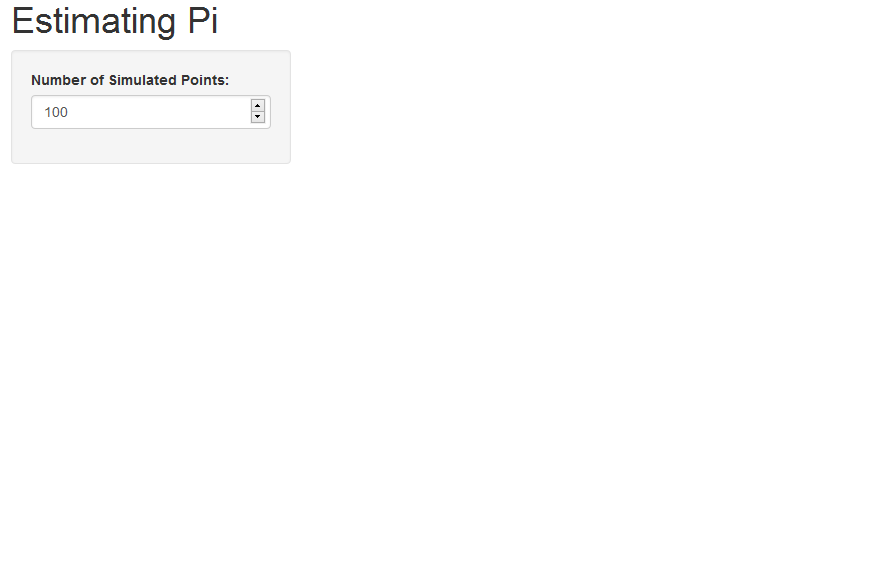
\includegraphics[width=.5\textwidth]{pictures/pi/input.PNG} 
   \caption{Shiny App with Inputs}
   \label{fig:appwithinputs}
\end{figure}
 
\noindent
Next we need to define the server-side of the application which will accept inputs and compute outputs.
Our server function will contain the code necessary to do this.
We first tell the function that we are creating a plot as an output, and we can create these outputs using the \texttt{renderPlot} and \texttt{renderText} command.

\begin{lstlisting}
    output\$monte <- renderPlot({
        
    })
    
    output\$estimate <- renderText({
    
    })
\end{lstlisting}
 
\noindent The goal of this program is to simulate hundreds points on a plot of a unit circle circumscribed in a square.
We need to generate x and y coordinates for these points, and then check if they fall within the circle.
To do this we will use the \textit{runif} command.
This command generates random deviates within a range of values for a certain number of observations.

\noindent We will set two variables, \texttt{x} and \texttt{y}, to store the \texttt{x} and \texttt{y} coordinates of the generated points.
Remember we want these values to lie between $-1$ and $1$ on the coordinate grid.
We want to run this simulation within the \texttt{renderPlot} and \texttt{renderText} functions so both outputs can access the result.
This can be done like so: 

\begin{lstlisting}
    output\$monte <- renderPlot({
        x <- runif(input\$simulate, min = -1, max = 1)
        y <- runif(input\$simulate, min = -1, max = 1
    })
    
    output\$estimate <- renderText({
        x <- runif(input\$simulate, min = -1, max = 1)
        y <- runif(input\$simulate, min = -1, max = 1
    })
   
\end{lstlisting}

\noindent The \texttt{input\$simulate} term is the number of simulations that the user inputs into the model.
This function will generate values between $-1$ and $1$ and store them in the \texttt{x} variable.
Now we have to test if these points lie within the circle. The equation of a circle is $x^{2}$ + $y^{2}$ = $r^{2}$.
This can be done using the \texttt{s.inside} command, which returns a $1$ or $0$ depending on if the point is inside the given boundary.
Then we want to find the ratio of the number of points within the circle to the number of total points and multiply this by $4$ to get an estimation of $\pi$. 

\begin{lstlisting}
     output\$monte <- renderPlot({
        x <- runif(input\$simulate, min = -1, max = 1)
        y <- runif(input\$simulate, min = -1, max = 1
        is.inside <- (x^2 + y^2) <= R^2
        estimation <- 4*sum(is.inside) / N
    })
    
    output\$estimate <- renderText({
        x <- runif(input\$simulate, min = -1, max = 1)
        y <- runif(input\$simulate, min = -1, max = 1
        is.inside <- (x^2 + y^2) <= R^2
        estimation <- 4*sum(is.inside) / N
    })
\end{lstlisting}

\noindent All we need to do now is to output the value of our estimation as well as the plot of the circle and the square.
To output the text, we can simply use a return function within the renderText environment under the rest of our code like so: 

\begin{lstlisting}
    return(c("Estimate of Pi:", estimation))
\end{lstlisting}
 
\noindent To plot the circle and the points, we use the \texttt{plot} command to place the randomly generated points on a grid, and use the \texttt{draw.circle} command to draw a circle.
To highlight which points are inside the circle we can color them blue, and the ones not inside will be colored red. 

\begin{lstlisting}
    plot(x, y, asp=1, xlim = c(-1,1), ylim = c(-1,1))
    draw.circle(0,0,1,nv=1000,lty=1,lwd=1)
    points(x[ is.inside], y[ is.inside], pch = 19, col = "blue")
    points(x[!is.inside], y[!is.inside], pch = 19, col = "red")
\end{lstlisting}

\noindent The above code should go in the \texttt{renderPlot} command under the previous code.
Now when the Shiny app is run your final project should like figure \ref{fig:Complete}. 

\begin{figure}[htbp!]
   \centering
   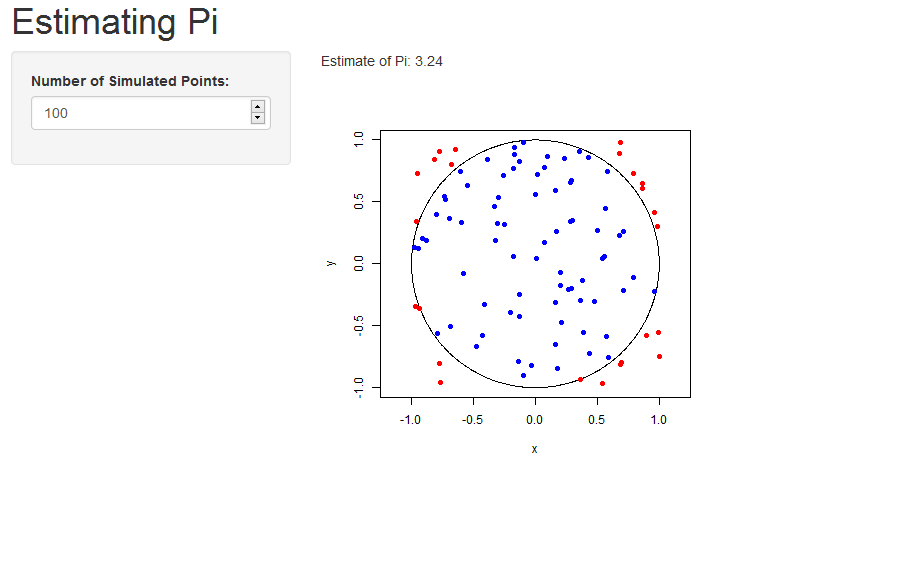
\includegraphics[width=0.5\textwidth]{pictures/pi/estimate.PNG} 
   \caption{Complete Estimating Pi Application}
   \label{fig:Complete}
\end{figure}

\noindent Your application is now complete!
Feel free to explore the approximations of $\pi$ as you increase or decrease the number of simulated points. 

\section{Deliverable}

For the final deliverable, the student should submit their code, along with a screenshot of the Shiny application using an instructor-defined number of simulated points.

\section{Teaching Code}

Students may use the framework below as a guide:

\begin{lstlisting}
#Student name
#Date
#EstimatingPi.R

#clean up and set the directory


#load libraries


#setting the server, code instructing R what to do with inputs


    #initialize objects
   
    
    #create plot
    
  
  #set up estimate routine  
  

#create graphics


#call shiny app


\end{lstlisting}

\section{Example Student Code}

The code that students submit should be similar to the example given below:

\begin{lstlisting}
#Ishaan Rao
#September 1, 2016
#EstimatingPi.R

#clean up and set the directory
rm(list=ls())
setwd("C:/Users/Ishaan/Documents/NCSSM 2015-2016")

#load libraries
library(shiny)
library(plotrix)

#setting the server, code instructing R what to do with inputs
server <- function(input, output) {
  output\$monte <- renderPlot({
    
    N <- input\$simulate
    R <- 1
    x <- runif(N, min = -R, max = R)
    y <- runif(N, min = -R, max = R)
    is.inside <- (x^2 + y^2) <= R^2
    estimation <- 4*sum(is.inside) / N
    
    #plot.new()
    #plot.window(xlim = 1.1 * R * c(-1, 1), ylim = 1.1 * R * c(-1, 1))
    plot(x, y, asp=1, xlim = c(-1,1), ylim = c(-1,1))
    draw.circle(0,0,1,nv=1000,lty=1,lwd=1)
    points(x[ is.inside], y[ is.inside], pch = 19, col = "blue")
    points(x[!is.inside], y[!is.inside], pch = 19, col = "red")
  })
  
  output\$estimate <- renderText({
    N <- input\$simulate
    R <- 1
    x <- runif(N, min = -R, max = R)
    y <- runif(N, min = -R, max = R)
    is.inside <- (x^2 + y^2) <= R^2
    estimation <- 4*sum(is.inside) / N
    
    return(c("Estimate of Pi:", estimation))
    
  })
}

ui <- shinyUI(fluidPage(
  headerPanel("Estimating Pi"),
  sidebarPanel(
    numericInput("simulate", "Number of Simulated Points:", 100, min = 100, max = 10000)
  ),
  mainPanel(
    textOutput("estimate"),
    plotOutput("monte", width = "400px", height = "400px")
  )
))

shinyApp(ui = ui, server = server)

\end{lstlisting}

\section{Further Readings}

To learn more about what Monte Carlo simulations are and their applications to a wide variety of problems visit \url{https://en.wikipedia.org/wiki/Monte\_Carlo\_method} or \url{http://www.palisade.com/risk/monte\_carlo\_simulation.asp}.

\noindent To learn more about the mathematical theory behind estimating $\pi$ visit \url{https://en.wikipedia.org/wiki/Approximations_of_\%CF\%80} or \url{http://polymer.bu.edu/java/java/montepi/MontePi.html}
